\chapter{Prototype System Implementation}
\label{chp:sys_imp}

\noindent In this chapter, it will cover development implementation progress of the prototype system along with explanation and analysis. The prototype system is implemented based on system design from chapter \ref{chp:sys_design}.

\section{WebRTC APIs Implementation}

\noindent \gls{webrtc} components are accessed with JavaScript APIs. Currently in development are the Network Stream \gls{api}, which represents an audio or video data stream, and the PeerConnection \gls{api}, which allows two or more users to communicate browser-to-browser. Also under development is a DataChannel \gls{api} that enables communication of other types of data for real-time gaming, text chat, file transfer, and so forth. Because the media server used in prototype system is not support for DataChannel yet, the DataChannel \gls{api} will not be covered in this section.

\begin{figure}
	\centering
    	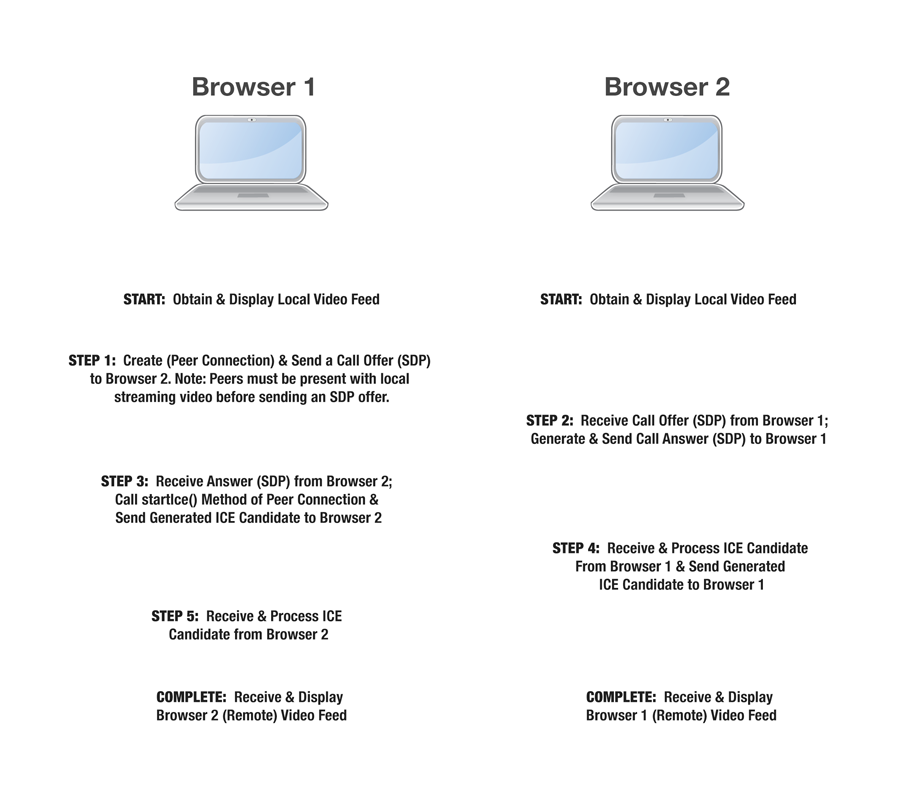
\includegraphics[height=0.50\textheight,natwidth=610,natheight=642]{figs/webrtc_diagram.png}
  	\caption{WebRTC two peer communication process\cite{mdn:p2pwebrtc}}
  	\label{fig:webrtc_diagram}
\end{figure}

\subsection{MediaStream API}

\par The MediaStream \gls{api} represents synchronized streams of media. For example, a stream taken from camera and microphone input has synchronized video and audio tracks. In order to obtain local media, the start step for both peers in Figure \ref{fig:webrtc_diagram} which is a communication process to set up call process from caller peer, the \gls{webrtc} \gls{api}s provide \textit{navigator.getUserMedia()} function to get the video and audio stream from user. For privacy reasons, a web application’s request for access to a user’s microphone or camera will only be granted after the browser has obtained permission from the user. Each MediaStream has an input, which might be a MediaStream generated by \textit{navigator.getUserMedia()}, and an output, which might be passed to a video element or an \textit{RTCPeerConnection}.
\par The \textit{getUserMedia()} method takes three parameters:

\begin{itemize}[topsep=-1em,parsep=0em,itemsep=0em]
 \item A constraints object.
 \item A success callback which, if called, is passed a MediaStream.
 \item A failure callback which, if called, is passed an error object.
\end{itemize}

\par The Code Snippet \ref{code:get_user_media} shows that how the prototype application implements \textit{getUserMedia()} function, it is encapsulated in \textit{WebRTCService} (service is a reusable business logic independent of views in prototype application regarding to AngularJs framework\footnote{AngularJS is an open-source web application framework, maintained by Google and community, that assists with creating single-page applications, one-page web applications that only require HTML, CSS, and JavaScript on the client side.\cite{wiki:angularjs}}).For the constraints object in parameters, the prototype application set 'audio' and 'video' value to true because it is necessary for the real-time communication application to have video and audio stream both.

\begin{lstlisting}[caption={Get User Media Stream function},label={code:get_user_media}]
var media_constraints = {audio: true,video: true};

function _setMediaStream(){
	WebRTCService.getUserMedia(media_constraints,
  								_handleUserMedia,
  								_handleUserMediaError);
  	console.log('Getting user media with constraints', 
  				media_constraints);
}
\end{lstlisting}

\par \textit{getUserMedia()} function is currently available in Chrome, Opera and Firefox. Almost all of the \gls{webrtc} \gls{api}s are slightly different based on different browsers implementation. In the Code Snippet \ref{code:webrtc_service}, there are two blocks to make all the set up process for FireFox and to make the same set up process for Google Chrome. Because \gls{webrtc} is not standard Web \gls{api} yet, so the implementation on different browsers are different and the \gls{webrtc} \gls{api}s names are slightly different in some browsers. For example, the \textit{RTCPeerConnection} \gls{api} in Firefox is \textit{mozRTCPeerConnection} but in Google Chrome it is \textit{webkitRTCPeerConnection}. In order to make the \gls{webrtc} application works on more browsers, the client side need to figure out which kind of browser is using on the machine then call the corresponding \gls{webrtc} \gls{api}s. Google provides a JavaScript shim called \textit{adapter.js}. It is maintained by Google, it abstracts away browser differences and spec changes. For Angularjs framework used by prototype application, then the \textit{WebRTCService} is implemented to be integrated with \textit{adapter.js} function to achieve the goal of compatibility.

\par However, the prototype application in this thesis will only focus on Google Chrome browser\footnote{Google Chrome is a freeware web browser developed by Google. It used the WebKit layout engine until version 27 and, with the exception of its iOS releases, from version 28 and beyond uses the WebKit fork Blink.\cite{wiki:google_chrome}} to simplify the development process because \gls{webrtc} lower level implementation on different browser s are different and hard to track the issues. Then most of the results in this thesis is based on the application performance of Google Chrome browser. The reason to choose Google Chrome browser rather than other browser because \gls{webrtc} is the technology rapidly pushed by Google and Google Chrome browser has the most market share in the world. As of March 2014, StatCounter estimates that Google Chrome has a 43\% worldwide usage share of web browsers, making it the most widely used web browser in the world.\cite{wiki:google_chrome} However, Google changes a lot to improve the performance of \gls{webrtc} on Google Chrome browser, then it makes the \gls{webrtc} \gls{api}s work different on different version of Google Chrome browser. In the Code Snippet \ref{code:webrtc_service}, from line 19 to line line 29 is the sample case to distinguish the difference among different version of Google Chrome to handle the \textit{RTCPeerConnection} \gls{ice} server constraint implementation.

\begin{lstlisting}[caption={WebRTCService.js in application client},label={code:webrtc_service}]
angular.module('webrtcDemo.services').
	factory('WebRTCService',function () {
		
		...

		function _setRTCElement() {

			if(navigator.mozGetUserMedia){
				...
			}else if(navigator.webkitGetUserMedia){
				...

			  // Creates iceServer from the url for Chrome.
			  _createIceServer = function(url, username, password) {
			    ...
			    if (url_parts[0].indexOf('stun') === 0) {
			      ...
			    } else if (url_parts[0].indexOf('turn') === 0) {
			      if (_webrtcDetectedVersion < 28) {
			        // For pre-M28 chrome versions use old TURN format.
			        var url_turn_parts = url.split("turn:");
			        iceServer = { 'url': 'turn:' + username + '@' + url_turn_parts[1],
			                      'credential': password };
			      } else {
			        // For Chrome M28 & above use new TURN format.
			        iceServer = { 'url': url,
			                      'credential': password,
			                      'username': username };
			      }
			    }
			    return iceServer;
			  };

			  ...
			}else{
				console.log("Browser does not appear to be WebRTC-capable");
			}

		}

		return {
			...
		}
	});	
	
\end{lstlisting}

\par Since \gls{webrtc} \gls{api}s is not standard \gls{api} yet, the prototype application in this thesis will not pay too much work-load on compatibility for different browsers platform. More detail about this issue will be discussed in the Chapter \ref{chp:future_work}.

\subsection{RTCPeerConnection API}

\noindent To set up peer connection, the \textit{RTCPeerConnection} \gls{api} sets up a connection between two peers. In this context, “peers” means two communication endpoints on the World Wide Web. Instead of requiring communication through a server, the communication is direct between the two entities. In the specific case of \gls{webrtc}, a peer connection is a direct media connection between two web browsers. This is particularly relevant when a multi-way communication such as a conference call is set up among three or more browsers. Each pair of browsers will require a single peer connection to join them, allowing for audio and video media to flow directly between the two peers. 

\par To establish peer connection, it requires a new \textit{RTCPeerConnection} object. The only input to the \textit{RTCPeerConnection} constructor method is a configuration object containing the information that \gls{ice}, will use to “punch holes” through intervening \gls{nat} devices and firewalls. The Code Snippet \ref{code:create_peer_connection} shows the create \textit{RTCPeerConnection} object and set three listener (\textit{onicecandidate},\textit{onaddstream},\textit{onremovestream}) to trigger the handlers to deal with the \gls{ice} candidate event and remote stream add/remove events.

\par The \textit{RTCPeerConnection} \gls{api} has two arguments to set, one is configuration object for peer connection and the other is constraint object (set transparent protocol and encryption) for peer connection, these value are shown in Code Snippet \ref{code:create_peer_connection} line 1 to line 10. In the showing case, the prototype is using \gls{stun} servers for different browser aspect, and set the \gls{rtc} channel encryption protocol to \gls{dtls}\footnote{In information technology, the Datagram Transport Layer Security (DTLS) protocol provides communications privacy for datagram protocols. DTLS allows datagram-based applications to communicate in a way that is designed to prevent eavesdropping, tampering, or message forgery.\cite{wiki:dtls}} and enable the \gls{rtc} DataChannel.

\par Because in Firefox, \gls{webrtc} media transparent channel is only based on \gls{dtls} protocol, and in latest version Google Chrome, it is support, then in the prototype application, it will use \gls{dtls} protocol to exchange the media stream.

\par There are two \gls{api}s to handle the \textit{IceCandidate} object which contains \gls{ice} information data. One is \textit{onicecandidate} listener to trigger the function to handle the new \textit{IceCandidate} data object. The other one is \textit{addIceCandidate} function, which is shown in the Code Snippet \ref{code:add_remote_ice}, to add the new \textit{IceCandidate} data object to the remote/local peer connection session description field. 

\begin{lstlisting}[caption={Create Peer Connection function},label={code:create_peer_connection}]
pc_config = WebRTCService.webrtcDetectedBrowser() === 'firefox' ?
  			{'iceServers':[{'urls':'stun:stun.services.mozilla.com'}]} :
  			{'iceServers':[{'urls': 'stun:stun.l.google.com:19302'}]};

pc_constraints = {
			  'optional': [
			    {'DtlsSrtpKeyAgreement': true},
			    {'RtpDataChannels': true}
			  ]
			};
			
function _createPeerConnection(){

	try {
		pc = WebRTCService.peerConnection(pc_config, pc_constraints);
		pc.onicecandidate = _handleIceCandidate;
		console.log('Created RTCPeerConnnection with:\n' +
		      '  config: \'' + JSON.stringify(pc_config) + '\';\n' +
		      '  constraints: \'' + JSON.stringify(pc_constraints) + '\'.');
	} catch (e) {
		console.log('Failed to create PeerConnection, exception: ' + e.message);
		alert('Cannot create RTCPeerConnection object.');
		return;
	}
	pc.onaddstream = _handleRemoteStreamAdded;
	pc.onremovestream = _handleRemoteStreamRemoved;

}
\end{lstlisting}

\begin{lstlisting}[caption={Add Remote IceCandidate function},label={code:add_remote_ice}]
var candidate = WebRTCService.RTCIceCandidate({
					    	sdpMLineIndex:data.content.label,
					    	sdpMid:data.content.id,
					    candidate:data.content.candidate
				});
pc.addIceCandidate(candidate);

\end{lstlisting}

\par In the step 2 of Figure \ref{fig:webrtc_diagram}, after the caller \textit{RTCPeerConnection} run \textit{createOffer()} function to send offer to callee through signaling channel, the callee need run \textit{createAnswer()} function to ask the \gls{stun}/\gls{turn} server to find the path for each other peer and create the answer with \gls{sdp} content. \gls{sdp} is intended for describing multimedia communication sessions for the purposes of session announcement, session invitation, and parameter negotiation. \gls{sdp} does not deliver media itself but is used for negotiation between end points of media type, format, and all associated properties.\cite{wiki:sdp} Before \textit{RTCPeerConnection} use \textit{createOffer()} function to send a \gls{webrtc} offer to the callee, it is required to be present with local streaming video, like Figure \ref{fig:webrtc_diagram} mentioned.

\par The sample \gls{sdp} from the prototype application is shown in Code Snippet \ref{log:webrtc_answer_sdp}. Line 2 in Code Snippet \ref{log:webrtc_answer_sdp} is the field 'o', it describes originator, session identifier, username, id, version number and network address. It usually means that where this package comes from. Line 7 and line 17 are field 'm', it describes media name and transport address. And line 11,12 and line 27,28 are the relevant lines for audio and video media field, they describes media filed 'candidate' attributes, in the sample case of Code Snippet \ref{log:webrtc_answer_sdp}, they are the \gls{ice} candidate from the \gls{stun}/\gls{turn} server. These are important fields regarding to the prototype system because they are used in XMS server and application server of the prototype system.

\begin{lstlisting}[caption={Sample \gls{webrtc} Answer \gls{sdp}},label={log:webrtc_answer_sdp}]
sdp: v=0
o=xmserver 1399363527 1399363528 IN IP4 10.254.9.135
s=xmserver
c=IN IP4 10.254.9.135
t=0 0
a=ice-lite
m=audio 49152 RTP/SAVPF 0 126
a=rtpmap:0 PCMU/8000
a=sendrecv
a=rtcp:49153
a=candidate:1 1 UDP 2130706431 10.254.9.135 49152 typ host
a=candidate:1 2 UDP 2130706430 10.254.9.135 49153 typ host
...
a=acfg:1 t=1
a=rtpmap:126 telephone-event/8000
a=fmtp:126 0-15
m=video 57344 RTP/SAVPF 100
b=AS:1000
a=rtpmap:100 VP8/90000
a=fmtp:100 max-fr=30; max-fs=1200
a=sendrecv
a=rtcp:57345
a=rtcp-fb:100 ccm fir
a=rtcp-fb:100 nack
a=rtcp-fb:100 nack pli
a=rtcp-fb:100 goog-remb
a=candidate:2 1 UDP 2130706431 10.254.9.135 57344 typ host
a=candidate:2 2 UDP 2130706430 10.254.9.135 57345 typ host
...
\end{lstlisting}

\par In the step 3 of Figure \ref{fig:webrtc_diagram}, the caller will receive the answer from callee and process it by adding the remote \gls{sdp} to \textit{RTCPeerConnection}, like the Code Snippet \ref{code:add_remote_ice}. By the meantime, the step 4 of Figure \ref{fig:webrtc_diagram}, the callee will receive the \gls{sdp} from caller with the \gls{ice} candidate information data, and process it the same way as caller does, add some to \textit{RTCPeerConnection} object by \textit{addIceCandidate()} function.

\par \gls{webrtc} clients (known as peers) also need to ascertain and exchange local and remote audio and video media information, such as resolution and codec capabilities. Signaling to exchange media configuration information proceeds by exchanging an offer and an answer using the \gls{sdp}. The \textit{createOffer()} function and \textit{createAnswer()} function both have callback function to handle the \gls{sdp} either to call \textit{setLocalDescription()} by caller or call \textit{setRemoteDescription()} by callee when callee gets the caller's \gls{sdp} from \gls{webrtc} offer. The Code Snippet\ref{log:webrtc_answer_sdp} shown is the \gls{webrtc} answer \gls{sdp} from the callee when the callee end-point decide to accept this conversion session.

\par Once the \textit{RTCPeerConnection} is established, the client need configure where the media or data to store and display if it is necessary. In the prototype application of this thesis, media stream will be displayed in a \gls{html5} tag called \textit{<video>}. It will only be shown when there is media stream in \textit{<video>} tag source.

\section{AngularJs framework Implementation}

\noindent As it described about AngularJs in Chapter \ref{chp:pre_study}, there are three layer components in the framework, view, controller and service. The files structure is shown in Appendix \ref{code:angularjs_structure}. Application has two main pages, \textit{login} page and \textit{phone} page. There are \textit{chatboard},\textit{contacts list}, \textit{contacts table}, \textit{dialpanel} and \textit{notification} user interface component block in \textit{phone} page. For each part of the application block, it has controller Javascript file and service Javascript file. Controller and service scripts are working with the \gls{html} view scripts. In this section, there will be one sample part of the prototype application client explained to understand how the AngularJs is used in prototype application.

\par The \textit{app.js} script shown in Code Snippet \ref{code:app_js} is the bootstrap script for AngularJs framework. It initializes the application module of AngularJs framework and declare the dependencies which will be used in the application.

\par The contact table component in \textit{phone} page of the application is structured in four scripts, \textit{contactTable.jade} script in Code Snippet \ref{code:contact_table}, \textit{ContactTableDirective.js} script in Code Snippet \ref{code:contact_table_dir}, \textit{ContactsCtrl.js} script in Code Snippet \ref{code:contact_ctrl} and \textit{GoogleAPIService.js} script in Code Snippet \ref{code:google_api}. It provides the application contacts information in advanced functioning table and search function in text input filed.

\subsection{app.js Script (AngularJs Bootstrap)}

\par The \textit{app.js} script shown in Code Snippet \ref{code:app_js}, it declares the application level module which depends on different filters, modules and services. The modules \textit{webrtcDemo.services}, \textit{webrtcDemo.controllers}, \textit{webrtcDemo.directives} and \textit{webrtcDemo.filters} are the customized modules implemented for prototype application. The rest of the module which are included as dependencies are third party AngularJs modules used in the prototype application. AngularJs developer community is quite active community, there are many useful open sourced projects or modules can be just included for using in the prototype application.

\par In the prototype application code, it used to set the application routing map. There are two main pages, one is \textit{login} page with "/login" \gls{url} and the other one is \textit{phone} page with "/chat" \gls{url}. The Angular controllers which are bind with these page view are also declared in \textit{\$routeProvider} service. And the default \gls{url} is set to "/login" to make sure if user has not logged in the system, he need to input the user credential to log himself. 

\label{app:app_js}
\begin{lstlisting}[caption={app.js in application client},label={code:app_js}]
angular.module('webrtcDemo', [
    ...
  'webrtcDemo.services',
  'webrtcDemo.controllers',
  'webrtcDemo.directives',
  'webrtcDemo.filters'
]).
config(function ($routeProvider, $locationProvider, $httpProvider) {
  $routeProvider.
    when('/chat', {
      templateUrl: 'partials/phoneView',
      controller: 'PhoneViewCtrl'
    }).
    when('/login',{
      templateUrl: 'partials/login',
      controller: 'LoginViewCtrl'
    }).
    otherwise({
      redirectTo: '/login'
    });

  ...
  });

\end{lstlisting}

\subsection{contactTable.jade Script (View)}

\par The \textit{contactTable.jade} script is the view component of the AngularJs. It is a Jade\footnote{Jade is a high performance template engine heavily influenced by Haml and implemented with JavaScript for node.\cite{github:jade}} script file. The template engine used on Node.js in prototype application is Jade which provides more clear way to program \gls{html} node template scripts. In the Code Snippet \ref{code:contact_table}, Jade has the same node name as normal node template engine \gls{ejs} and some Angular directives in the template. For example, at line 2 in Code Snippet \ref{code:contact_table}, the \textit{angucomplete-alt} directive is a third party Angular directive to provide auto-completion features in \gls{html} \textit{<input>} text tag. The different attributes in the \textit{angucomplete-alt} node is to set some configuration to this directive, like the attribute files \textit{local-data} is the array data to search for content as auto-complete reference.

\par Moreover, AngularJs itself provides native Angular directive as well. For instance, at line 11 in Code Snippet \ref{code:contact_table}, the attribute \textit{ng-class} is a native Angular directive attribute, it provides the \gls{css}\footnote{Cascading Style Sheets (CSS) is a style sheet language used for describing the look and formatting of a document written in a markup language.\cite{wiki:css}} change to some specific \gls{css} class name when some certain value matches in AngularJs expression. At line 11, the \textit{<tr>} tag's \gls{css} attributes will be success class only if the boolean value of \textit{item.online} is \textit{true}.

\par AngularJs provides two-way data module binding in the template and controller. Line 17 in the Code Snippet \ref{code:contact_table}, \textit{\{\{item.number\}\}} is the Angular template to display the \textit{number} property value of \textit{item} object in the \gls{html} template. And line 14 is the example of Angular template integrated with Angular filter, the third-party filter \textit{iif} here is the filter to check the \textit{\{\{item.online\}\}} value if it is \textit{true} or \textit{false}. If it is \textit{true} then it will show \textit{Online} string text in the \gls{html} template otherwise it will show \textit{Offline} string text. The syntax here is quite similar to any other programming language.

\begin{lstlisting}[caption={contactTable.jade in application client},label={code:contact_table}]
div(id = "contactTable")
	angucomplete-alt(id="contactSearch",
		...
		local-data="contactsHolder.contacts",
		...)
	tabset
		tab(heading = "Conacts")
			table(id = "contacts", at-table, at-paginated, at-list="contactsHolder.contacts | orderBy:online", at-config="config",class="table table-hover table-striped table-condensed" )
				thead
				tbody
					tr(ng-class = "{success: item.online}", ng-init = "item.hvor = false", ng-mouseenter = "contactHvor(item)", ng-mouseleave = "contactHvor(item)")
						...
							p(ng-hide = "item.hvor").
								{{item.online | iif : "Online" : "Offline" }}
                        ...
							p
								| Telephone : {{item.number}}
			...
\end{lstlisting}

\subsection{ContactTableDirective.js Script (Customized Directive)}

\par After creating the view of contact table component, it is necessary to make a customized directive to bind controller to the view. It is called \textit{Directive} in AngularJs, the \textit{ContactTableDirective.js} script is shown in Code Snippet \ref{code:contact_table_dir}. From line 1 to line 12 is the directive declaration, it sets the \textit{templateUrl} to 'partials/contactTable' which is the view component of contact table file path and binds the controller which name \textit{ContactsCtrl} to the view component. The \textit{restrict} filed in the directive is to set the template type for \textit{ContactTableDirective}, in the Code Snippet \ref{code:contact_table_dir} line 5, it means this directive is a \gls{html} element template, it can be used as normal \gls{html} element by using name 'contact-table'.

\par From line 14 to line 19 is the Angular filter declaration, it is a filter name \textit{iif}, the only function it does is to check the \textit{input} value and return \textit{trueValue} if \textit{input} is \textit{true} otherwise return \textit{falseValue}. The usage is described in previous section in line 14 of the Code Snippet \ref{code:contact_table}.

\begin{lstlisting}[caption={ContactTableDirective.js in application client},label={code:contact_table_dir}]
angular.module('webrtcDemo.directives').
	directive('contactTable',function () {

		return{
			restrict: 'E',
			replace: true,
			scope: true,
			templateUrl: 'partials/contactTable',
			controller: 'ContactsCtrl'
		};

	});

angular.module('webrtcDemo.filters').
	filter('iif', function () {
   return function(input, trueValue, falseValue) {
        return input ? trueValue : falseValue;
  };
});
\end{lstlisting}

\subsection{ContactsCtrl.js Script (Controller)}

\par The controller in AngularJs is to control the user interface logic and bridge the data business logic from the services to the user interface views. The example controller in Code Snippet \ref{code:contact_ctrl} controls the contactTable view directive and get data from GoogleAPIService. At the line 2 of Code Snippet \ref{code:contact_ctrl}, in the controller construction function, there are several services arguments. They are the services this controller will use in the application, one of them is \textit{GoogleAPIService} which is related to the contacts information data. The contactTable view directive need contacts information data to show in the \gls{html} template. And \textit{storage} is another service provides \\textit{localstorage} function in \gls{html5} application. This service is used to store the contacts information data locally to make user no need to import his Google contacts information all the time. This function is implemented at line 23 of the Code Snippet \ref{code:contact_ctrl}.

\par At line 5 of the Code Snippet \ref{code:contact_ctrl}, it is the function \textit{\$scope.importContacts}, the reason this function is under \textit{\$scope} object is because this function is directly triggered by one \gls{ui} button. In this function, there are two Javascript promise function from the \textit{GoogleAPIService}. One is \textit{GoogleAPIService.oAuth()} function which is to ask user to get Google \gls{api} permission to query the Google Contacts \gls{api}. The other one is after get the Google \gls{api} permission to query the contacts information data by Google Contacts \gls{api}.

\par \textit{Promise} object is the new concept in the Javascript and AngularJs. The core idea behind promises is that a promise represents the result of an asynchronous operation. A promise is in one of three different states:\cite{website:promise}
\begin{itemize}[topsep=-1em,parsep=0em,itemsep=0em]
 \item \textbf{Pending} - The initial state of a promise.
 \item \textbf{Fulfilled} - The state of a promise representing a successful operation.
 \item \textbf{Rejected} - The state of a promise representing a failed operation.
\end{itemize}
It is a great concept in the AngularJs. Since everything in Javascript is asynchronous operation, then promise object function is used to deal with the function calling after previous asynchronous operation success. The implementation of these two promise functions will be covered in the next section.

\par From line 9 to line 15 is the process to filter out the useful information from the response data to get the correct contact information into \textit{contact} object, then push them one by one into a \textit{contact} object array in order to be used by contact table view component.

\begin{lstlisting}[caption={ContactsCtrl.js in application client},label={code:contact_ctrl}]
angular.module('webrtcDemo.controllers').
	controller('ContactsCtrl',function ($scope,$location,WebSocketService,GoogleAPIService,storage,$filter) {
		...
		
		$scope.importContacts = function(){
			$scope.contactsHolder.contacts = [];
			GoogleAPIService.oAuth().then(function(token){
				GoogleAPIService.queryContacts(token).then(function(data){
					angular.forEach(data.feed.entry,function(person, key){
						if(person['gd$phoneNumber']){
							var contact = {
								name: person.title['$t'],
								number: person['gd$phoneNumber'][0]['$t'],
								online: false
							}

							...

						}
					});

					storage.set('contactList-' + username,$scope.contactsHolder.contacts);

				});
			});
		}

	});
\end{lstlisting}


\subsection{GoogleAPIService.js Script (Service)}

\par AngularJs service provides most of the business logic of the application. Like the sample code shown in Code Snippet \ref{code:google_api}, it provides interfaces of Google \gls{api} to the controller. There are two interfaces in the \textit{GoogleAPIService.js} script. One is Google authorization login and get the user permission, the other one is fetching Google contacts information from the Google Contacts \gls{api}.

\par From line 4 to line 20 in Code Snippet \ref{code:google_api}, it is the promise function, \textit{\_authLogin()}, to get Google authorization token in order to call any Google \gls{api} later. It uses \textit{\$q} service from AngularJs to provide \textit{deferred} \gls{api} and \textit{prmoise} \gls{api}. The purpose of the deferred object is to expose the associated Promise instance as well as \gls{api}s that can be used for signaling the successful or unsuccessful completion, as well as the status of the task.The purpose of the promise object is to allow for interested parties to get access to the result of the deferred task when it completes.\cite{angular:q} At line 5 and line 23 is the code to create a new instance of deferred and a new promise instance. From line 7 to 10, it is the configuration object for Google \gls{api} authorization. The \textit{gapi} object is from the Google \gls{api} Javascript client script included in \textit{index.jade} shown in Code Snippet \ref{code:include_googleapi}.

\begin{lstlisting}[caption={Include Google API Javascript file in Index.iade},label={code:include_googleapi}]
script(src='https://apis.google.com/js/client.js' type='text/javascript')
\end{lstlisting}

\par Since application only need to get permission form user Google Contacts, then the scope is set to \url{https://www.google.com/m8/feeds} and the client\_id is got from the Google App Engine (\url{https://console.developers.google.com}). Developer need to create his own Google App project then set the \gls{api}s which the project will ask user permission to use and the credentials used for client or web service. In the prototype system, it is the web application client to use the Google Contacts \gls{api} then there is a client \gls{oauth} 2.0\footnote{OAuth is an open standard for authorization. OAuth provides client applications a 'secure delegated access' to server resources on behalf of a resource owner.OAuth 2.0 is the next evolution of the OAuth protocol and is not backwards compatible with OAuth 1.0. OAuth 2.0 focuses on client developer simplicity while providing specific authorization flows for web applications, desktop applications, mobile phones, and living room devices.\cite{wiki:oauth}} credential created on Google App project.

\par Then the \textit{gapi} object call \textit{auth.authorize()} function with the configuration object to get authorization token. At line 15, when the asynchronous process is finished, \textit{deferred} object to call \textit{resolve} function to send the token object back to the promise \textit{then} function at line 7 in Code Snippet \ref{code:contact_ctrl} which is mentioned at previous section.

\par From line 22 to line 34 in Code Snippet \ref{code:google_api} is another promise function, \textit{\_fetchContacts()} , to fetch the Google contacts information data after getting user permission to use their Google service data. This function makes a \gls{http} request in \gls{jsonp} to fetch all the contacts information from Google Contacts \gls{api}. \gls{jsonp} is a communication technique used in JavaScript programs running in web browsers to request data from a server in a different domain, something prohibited by typical web browsers because of the same-origin policy. \gls{jsonp} takes advantage of the fact that browsers do not enforce the same-origin policy on \textit{<script>} tags. Th reason the application uses \gls{jsonp} in \gls{http} request is that web application is host in one origin domain and Google \gls{api} server is in another origin domain, it is cross domain request when prototype application request for data from Google \gls{api} server. And Google \gls{api} server does not support cross domain request, but with \gls{jsonp} it is allowed to have cross origin domain resources sharing.

\par The \textit{\_fetchContacts()} function uses the same mechanism as \textit{\_authLogin()} function described above to make promise function, it returns contacts information data from Google Contacts \gls{api}.

\begin{lstlisting}[caption={GoogleAPIService.js in application client},label={code:google_api}]
angular.module('webrtcDemo.services').
	factory('GoogleAPIService', function ($q,$http,storage) {

		function _authLogin(){
			var deferred = $q.defer();

			var config = {
		      'client_id': 'xxxxxxxxxxxxxxx.apps.googleusercontent.com',
		      'scope': 'https://www.google.com/m8/feeds'
		    };
	    gapi.auth.authorize(config, function() {

	      console.log('login complete');
	      console.log(gapi.auth.getToken());
	      deferred.resolve(gapi.auth.getToken());

	    });

	    return deferred.promise;
		}

		function _fetchContacts(authToken){
			...
			
			$http.jsonp(url).
	    success(function(data, status, headers, config) {
	      deferred.resolve(data);
	    }).
	    error(function(data, status, headers, config) {
	      deferred.reject('GoogleAPIService:queryContacts:Failed');
	    });

			return deferred.promise;
		}

		...
	});
\end{lstlisting}

\section{Socket.IO Implementation}

\noindent In the prototype system, web application client and application server are communicating over WebSocket shown in Figure \ref{fig:system_network}. There are two main intentions to have the signaling channel over WebSocket. One is to signaling for \gls{webrtc} \gls{ice} candidate exchange and the other one is to exchange the communication data (text message, files). Unlike \gls{http}, WebSocket provides for full-duplex communication. Additionally, Websocket enables streams of messages on top of \gls{tcp}. \gls{tcp} alone deals with streams of bytes with no inherent concept of a message. Before WebSocket, port 80 full-duplex communication was attainable using Comet channels; however, Comet implementation is nontrivial, and due to the \gls{tcp} handshake and \gls{http} header overhead, it is inefficient for small messages. WebSocket protocol aims to solve these problems without compromising security assumptions of the web.\cite{wiki:websocket}

\subsection{Server Side Implementation}

\par The Code Snippet \ref{code:server_socket}, it is implementation of Socket.IO on the application server. From line 1 to line 13, they are the intialization process of the Socket.IO on Node.js. At line 10, it means that when the client binds with the application server through WebSocket, the listener start in handler function \textit{\_handlerSocket()}. The WebSocket channels and usage is shown in Table \ref{tab:websocket}.

\par At line 27 in Code Snippet \ref{code:server_socket}, \textit{socket} object is created by the Socket.IO framework whenever one client connects with the server through WebSocket. The \textit{listener} function is implemented in the same pattern \textit{socket.on()}. There are two arguments taken by this function. The first one is the channel name, at line 27, it is \textit{sip}, and second argument is callback function when this channel got any socket message. This callback function also take one argument which is the message data sent by the client.

\par At line 74 in Code Snippet \ref{code:server_socket}, it is implementation for server to send socket message back to the client through WebSocket in Socket.IO framework. \textit{socket.emit()}, this function takes two arguments, the first one is the WebSocket channel name and second one is the socket message data object. All the socket message data is formatted in \gls{json} because it is easier for both client and server side to resolve these message data.

\begin{table}
\caption{\label{tab:websocket}: Socket.IO Listening Channels in Code Snippet \ref{code:server_socket}}
\centering
\begin{tabular}{| c | p{3cm} | p{5.5cm} |}
\hline
 WebSocket Channel & Message Data Type & System Function \\ \hline
 \multicolumn{1}{ |c| }{\multirow{3}{*}{\gls{sip}} } & \multicolumn{1}{ | p{3cm} | }{register(line 30 - 37)} &  Web application login page \gls{sip} registeration message to \gls{sip} server\\ \cline{2-3}
 \multicolumn{1}{ |c  }{} & \multicolumn{1}{ | p{3cm} | }{invite(line 38 - 107)} & Web application client invite \gls{sip} client message \\ \cline{2-3}
 \multicolumn{1}{ |c  }{} & \multicolumn{1}{ | p{3cm} | }{answerInvite(line 108 - 167)} & Web application client get INVITE \gls{sip} message from \gls{sip} client and answer it \\ \cline{1-3}
 \multicolumn{1}{ |c| }{\multirow{5}{*}{\gls{webrtc}} } & \multicolumn{1}{ | p{3cm} | }{register(line 248 - 283)} &  Web application client finish login with \gls{sip} credential and get user permission to use \textit{getUserMedia()} function and register client itself on application server for WebSocket use \\ \cline{2-3}
 \multicolumn{1}{ |c  }{} & \multicolumn{1}{ | p{3cm} | }{offer(line 218 - 247)} & Web application client send offer message to appliction server to create call resource on XMS media server \\ \cline{2-3}
 \multicolumn{1}{ |c  }{} & \multicolumn{1}{ | p{3cm} | }{answerInvite(line 173 - 194)} & Web application client get INVITE message from \gls{webrtc} client and answer it \\ \cline{2-3}
 \multicolumn{1}{ |c  }{} & \multicolumn{1}{ | p{3cm} | }{endCandidate(line 284 - 317)} & Web application client finish get \gls{ice} candidate from \gls{stun}/\gls{turn} server then application send \gls{http} request to XMS media server with final \gls{sdp} \\ \cline{2-3}
 \multicolumn{1}{ |c  }{} & \multicolumn{1}{ | p{3cm} | }{hangup(line 321 - 551)} & Web application client send hangup messge to hangup iteself from the current conference \\ \cline{1-3}
 \multicolumn{1}{ |c| }{\multirow{2}{*}{message} } & \multicolumn{1}{ | p{3cm} | }{\gls{im}(line 566 - 582)} &  Web application send instance message to application server in order to broadcast to all the clients in current conference\\ \cline{2-3}
 \multicolumn{1}{ |c  }{} & \multicolumn{1}{ | p{3cm} | }{\gls{sms}(line 584 - 594)} & Web application client send \gls{sms} to \gls{sip} client \\ \cline{1-3}
 disconnect & *(line 604 - 639) &  Web application client disconnect from the application server\\ \hline
\end{tabular} 
\end{table}

\subsection{Client Side Implementation}

\par Since Socket.IO library is a library to make the communication channel between server and client, besides server side implementation, there is client side implementation(shown in Code Snippet \ref{code:client_socket} ) which is correspond to the server side implementation.

\par The client side Socket.IO implementation is quite similar as the server side implementation mentioned above. The socket message event listener is implemented as the same pattern like line 3 in Code Snippet \ref{code:client_socket}. Moreover, at line 67, \textit{socket.emit()} function is used for client to send socket message through WebSocket to server in Socket.IO framework. In this way, the client has same WebSocket channels listed in Table \ref{tab:websocket} and sends the related data type to the server to request server to run some corresponding process.
 

\section{SIP Implementation on Application Server}

\noindent There are not many \gls{sip} stack \gls{npm}\footnote{npm is the official package manager for Node.js. As of Node.js version 0.6.3, npm is bundled and installed automatically with the environment. npm runs through the command line and manages dependencies for an application. It also allows users to install Node.js applications that are available on the npm registry.\cite{wiki:npm}} module made for Node.js. After a lot of research, this prototype system will use a simple \gls{sip} module(sip.js,\url{https://www.npmjs.org/package/sip}) on Node.js. It implements tranaction and transport layers as described in RFC3261. This library is still maintained by its author although the developer of this library is not so active during this thesis writing period. But this library is the most fit library for Node.js.

\par Most of example of sip.js library usage is to be implemented as a \gls{sip} registration server or proxy server. Then the most of the interfaces provided by sip.js library are design for redirecting all the \gls{sip} message and \gls{sip} register request. Although sip.js library provides \gls{sip} stack for Node.js and lower layer transportation on \gls{sip} protocol interface, it is not designed for manually generating different \gls{sip} message request to \gls{sip} server. Most of the \gls{sip} implementation of prototype application server have to be handled with all the \gls{sip} message generation issues by its own implementation Javascript code which is shown in Code Snippet \ref{code:sipjs}. These implementation is made based on the reference of RFC3261 and Wireshark\footnote{Wireshark is a free and open-source packet analyzer. It is used for network troubleshooting, analysis, software and communications protocol development, and education. Originally named Ethereal, in May 2006 the project was renamed Wireshark due to trademark issues.\cite{wiki:wireshark}} trace log of the \gls{sip} soft-phone application\footnote{A softphone is a software program for making telephone calls over the Internet using a general purpose computer, rather than using dedicated hardware.\cite{wiki:softphone}} (Zoiper).

\subsection{SIP Request Message Implementation}

\par As mentioned in Chapter \ref{chp:intro}, there will be \textit{REGISTER},\textit{INVITE},\textit{ACK},\textit{CANCEL} and \textit{BYE} \gls{sip} message request implemented in application server to provide normal \gls{webrtc} browser client have the \gls{sip} communication ability. Otherwise the sip.js library provides mostly used \gls{sip} response, it is no need to modified these response when application server need to send the \gls{sip} response back to client.

\par From line 24 to line 41 of Code Snippet \ref{code:sipjs} , it is the code block for generating \textit{REGISTER} \gls{sip} message request. It is implemented regarding to RFC3261. The important part of this block implementation is the header of \textit{REGISTER} \gls{sip} message. There are \textit{call-id},\textit{cseq},\textit{from},\textit{to},\textit{contact} fields need to be set in the header. \textit{call-id} contains a globally unique identifier for this call, generated by the combination of a random string and the client's host name or \gls{ip} address. The combination of the \textit{to} tag, \textit{from} tag, and \textit{call-id} completely defines a peer-to-peer \gls{sip} relationship between two end points and is referred to as a dialog. \textit{cseq} or Command Sequence contains an integer and a method name. The \textit{cseq} number is incremented for each new request within a dialog and is a traditional sequence number. For the prototype application server, the \textit{cseq} number is increased (shown at line 319 of Code Snippet \ref{code:sipjs} ) when the \gls{sip} \textit{REGISTER} request is unauthorized then application server need to send another \gls{sip} \textit{REGISTER} request with authorization information. This process is implemented from line 315 to line 350 in Code Snippet \ref{code:sipjs}. Moreover, since the return 200 \textit{OK} \gls{sip} response with the limited expired time for this \textit{REGISTER} session, at line 331, the application server set up a timer to re-register the client after the expired time. \textit{to} contains a display name and a \gls{sip} or \gls{sip}s \gls{uri} towards which the request was originally directed. \textit{from} also contains a display name and a \gls{sip} or \gls{sip}s \gls{uri} that indicate the originator of the request. This header field also has a tag parameter containing a random string that was added to the \gls{uri} by the application server. It is used for identification purposes. \textit{contact} contains a \gls{sip} or \gls{sip}s \gls{uri} that represents a direct route to contact client, usually composed of a username at a \gls{fqdn}. It is important to use application server public \gls{ip} address and port since all the client \gls{sip} request message and \gls{sip} response need to be send to application server to trigger other process for the prototype use in the system.

\begin{lstlisting}[caption={ACK Alice -> Bob Sample \cite{rfc:3665}},label={code:ack_sample}]
   ACK sip:bob@client.biloxi.example.com SIP/2.0
   Via: SIP/2.0/TCP client.atlanta.example.com:5060;branch=z9hG4bK74bd5
   Max-Forwards: 70
   From: Alice <sip:alice@atlanta.example.com>;tag=9fxced76sl
   To: Bob <sip:bob@biloxi.example.com>;tag=8321234356
   Call-ID: 3848276298220188511@atlanta.example.com
   CSeq: 1 ACK
   Content-Length: 0
\end{lstlisting}

\par During the development, there is a bug issue found in the sip.js library when it regards to implement the \textit{ACK} \gls{sip} message when an \textit{INVITE} \gls{sip} message got accepted (200 \textit{OK} message). The example \gls{sip} \textit{ACK} message is from RFC3665(\url{http://tools.ietf.org/html/rfc3665}) shown in Code Snippet \ref{code:ack_sample}. When implementing this \gls{sip} message in sip.js, the \gls{uri} field at line 78 of Code Snippet \ref{code:sipjs} need to set the port number on it to force this \gls{sip} message send to correct \gls{sip} protocol port on the \gls{sip} server which is regarding to line 2 of Code Snippet \ref{code:ack_sample} in most \gls{sip} server case including the target server in this prototype system. Then the implementation of this process, shown from line 72 to line 75 is to check if the contact \gls{uri} of the \gls{sip} response header has port number or not. If there is no port number in it, it need to set the \gls{uri} with the \textit{5060} port number which is the target \gls{sip} server \gls{udp} port with \gls{sip} protocol implementation (it is implemented in same way as most \gls{sip} server).

\subsection{SIP Message Listener and Handler Implementation}

\par The application server in the prototype system does not only create \gls{sip} request message and send them to \gls{sip} server, but also listens to the \gls{sip} request/response message from the \gls{sip} server.

In Code Snippet \ref{code:sipjs}, from line 198 to line 307, it is the initialization function for \gls{sip} gateway on application server. There are two parts in this code block. The first part is from line 199 to line 214 in Code Snippet \ref{code:sipjs}, it is the initialization of the \gls{sip} stack on application server \textit{5060} port. It configures the \gls{sip} stack on host \gls{ip} address and host port number, also initializes the registration array for sip client credentials. Then at line 206, the function \textit{sip.start()} is to start the \gls{sip} stack listener on these \gls{sip} gateway configuration. 

\par The second part of the code in in Code Snippet \ref{code:sipjs}, from line 215 to line 307, it is the \gls{sip} listener to handle different \gls{sip} request and \gls{sip} response. Since the communication protocol between \gls{webrtc} browser clients and application server is based on WebSocket not \gls{sip}. Then the \gls{sip} message to the application server is from the \gls{sip} server on the traditional telephony network. The \textit{rq} object in Code Snippet \ref{code:sipjs} is the request/response \gls{sip} stack object on application server. It is the same message object when the application send to \gls{sip} server in sip.js library. Then in the code block of this part, it is necessary to check the \textit{method} parameter of \textit{rq} object to find out which type message it is.

\par For example, from line 229 to line 259 in Code Snippet \ref{code:sipjs}, it is the code block when there is \gls{sip} \textit{INVITE} request from the \gls{sip} server. It means that there is one \gls{sip} client want to call the other \gls{webrtc} browser client in the prototype system. The application firstly send back a \textit{Trying} \gls{sip} response back to the \gls{sip} server (at line 234 - 235 in Code Snippet \ref{code:sipjs}) to notice that the application server tries to find out if this contact number is online in the prototype system by using the \textit{sip.makeResponse} function. Then if the contact number is online in the prototype sytem, the application stores some necessary information data from the \textit{INVITE} request (at line 238 - 241 in Code Snippet \ref{code:sipjs}), and broadcast an internal event (\textit{SIPREMOTE}) by \textit{EventEmmitter} (init at line 12 in Code Snippet \ref{code:sipjs}) from \textit{events} module in Node.js framework. This event is used to let \textit{socket} block of application server notice the remote \gls{sip} event then send necessary WebSocket message to the client in order to notice the end point user about the \gls{sip} messages(in \textit{INVITE} example, the socket handler function is shown in Code Snippet \ref{code:socket_remote_invite} ).

\begin{lstlisting}[caption={SIPREMOTE event handler for INVITE message},label={code:socket_remote_invite}]
function _handlerSip(){
  gw.on('SIPREMOTE', function (data) {
      switch(data.type){
          ...
          
          case 'INVITE':

            var client = clients[data.content.toNumber];

            if(client.inConference){

              gw.sendBusy(data.content.inviteRequest,function(rs){
                console.log('client number: ' + data.content.toNumber + 'is in the conference');
              });

            }else{
              var id = uuid.v1();
              callRequests[id] = _createCallRequest(id);

              client.callreq_id = id;
              client.endIceCandidate = false;

              sipClients[data.content.fromNumber] = _createSipClient(data.content.fromNumber);
              var sip = sipClients[data.content.fromNumber];
              sip.callreq_id = id;

              callRequests[id].caller = sip;
              callRequests[id].callee = client;
              callRequests[id].sipInviteRequest = data.content.inviteRequest;

              //console.log('SIPREMOTE:INVITE: remote sip sdp' + data.content.inviteRequest.content);

              xmsManager.createXMSCall({
                callType: 'sip',
                sdp: data.content.inviteRequest.content
              },function(remote_xmsSDP,remote_id){
                sip.remote_xmsSDP = remote_xmsSDP;
                sip.remote_identifier = remote_id;

                client.socket.emit('sip',{
                  type: "createRTCoffer",
                  inComingNumber: data.content.fromNumber,
                  callDirection: 'outbound'
                });

                gw.sendAnswer(data.content.toNumber,
                  data.content.inviteRequest,
                  remote_xmsSDP,
                  function(){
                    console.log('200 ok answer sent');
                });

              });
            }
        
            break;
          
          ...
      }
  }
\end{lstlisting}

\par In Code Snippet \ref{code:socket_remote_invite}, at line 10, it checks if the receiver of this \gls{sip} \textit{INVITE} message is in the conversation already. If not, it will send \textit{createXMSCall} request to XMS media server to create a new call resource for the \gls{sip} client and send WebSocket message about this invite to the \gls{webrtc} target client.(from line 33 to line 54 in Code Snippet \ref{code:socket_remote_invite}) The integration with XMS media server of application server will be discussed more in the later chapter.

\section{XMS Media Server Integration on Application Server}

\noindent XMS media server is used as media gateway in the prototype system, the main functions of it are to create call conference session for multiple clients and to convert between \gls{webrtc} \gls{sdp} and \gls{sip} \gls{sdp} in order to bridge the \gls{webrtc} clients and \gls{sip} clients on \gls{rtp} channel.

\par Since the integration is only between application server and XMS media server, using \gls{rest}ful\footnote{Representational state transfer (REST) is a software architectural style consisting of a coordinated set of architectural constraints applied to components, connectors, and data elements, within a distributed hypermedia system. REST ignores the details of component implementation and protocol syntax in order to focus on the roles of components, the constraints upon their interaction with other components, and their interpretation of significant data elements.\cite{wiki:restful}} communication based on \gls{http} is a good solution to the working scenario and it is supported by XMS media server and Node.js framework on application server. The detail working flow of the prototype system integrated with XMS media server is shown in Figure \ref{fig:chrome2xms}.

\par In the process of single call from \gls{webrtc} client to \gls{sip} client, the application server need to send \textit{INVITE} message with \gls{webrtc} \gls{sdp} of browser client to XMS media server(create call request) in order to request XMS media server to create \gls{webrtc} call resource and get the \gls{sdp} of this newly created call resource from XMS media server. After \gls{webrtc} and newly created call resource connected in the \gls{rtp} channel, application server sends \textit{INVITE} message without \gls{sdp}(create call request) to XMS media server in order to create \gls{sip} call resource and use the return \gls{sdp} to send \gls{sip} \textit{INVITE} message to \gls{sip} server to crate \gls{rtp} session with \gls{sip} client. At the end, application server sends \textit{join} request to XMS media server in order to joint these two created \gls{webrtc} call and \gls{sip} call resources in order to connect two different \gls{rtp} session channel. The process of multiple clients join a existing conference resource on XMS media server is a similar process as the single call example in Figure \ref{fig:chrome2xms}.

\begin{figure}
	\centering
    	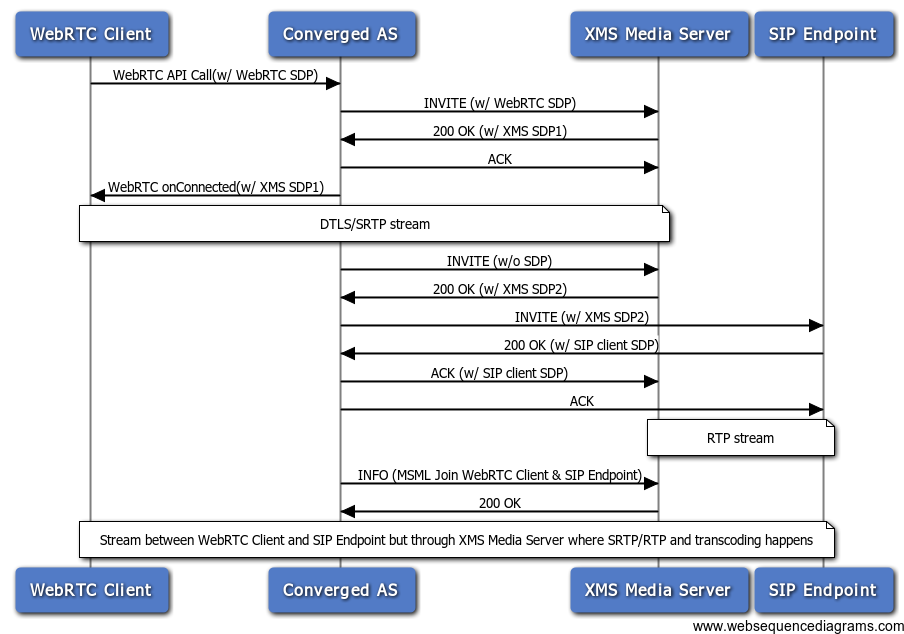
\includegraphics[width=0.95\textwidth,natwidth=610,natheight=642]{figs/chrome2xms.png}
  	\caption{Single Call from Browser to SIP Client}
  	\label{fig:chrome2xms}
\end{figure}

\par According to the documentation provided by Dialogic on XMS 2.1 \gls{rest}ful \gls{api}\cite{doc:xms_webapi}, it is only necessary to set \textit{encryption} field as \textit{dtls} and \textit{ice} as field \textit{yes} in the \gls{sdp} for \gls{webrtc} \gls{sdp} otherwise not set both fields for \gls{sip} \gls{sdp} when creating a call resource on XMS media server(shown at line 5-6 in Code Snippet \ref{code:xms}). It makes the interfaces on application not need to implemented differently for \gls{webrtc} and \gls{sip} clients.

\par In this sense, there are \textit{createXMSCall}, \textit{joinXMSCall}, \textit{updateLocalSDP}, \textit{createConference}, \textit{joinConference}, \textit{deleteXMSCall} and \textit{deleteXMSConference} interfaces(shown in Code Snippet \ref{code:xms} ) implemented on application server by the reference of XMS 2.1 RESTful API User's Guide \cite{doc:xms_webapi}.

\par Using \textit{createXMSCall} function as example of XMS integration implementation (from line 1 to line 48 in Code Snippet \ref{code:xms}), application server use \textit{http} Node.js module and \textit{xml2js} Node.js module to implement this interface. Regards to XMS 2.1 \gls{rest}ful \gls{api}, creating call resource on XMS media server is a \textit{POST} \gls{http} request with \gls{xml} request content. From line 2 to line 9 n Code Snippet \ref{code:xms} is to generate the \gls{xml} content. And at line 12, application call \textit{http.request()} function with the \textit{option} object and callback function. The request \textit{option} object has \textit{host},\textit{port},\textit{method},\textit{path},\textit{headers} fields need to be configured. The important part is the \textit{Content-length} is necessary in the headers field, it is the length of the \gls{xml} content. These are configured from line 13 to line 21 in Code Snippet \ref{code:xms}. In the callback function, application server need to check the response data from the \gls{http} \textit{POST} request. By using \textit{xml2js} module object \textit{xmlparser} to parse the \gls{xml} data into \gls{json}. From line 32 to line 34, it is the process to strip the useful data \gls{sdp} from the response data. After the other process from line 36 to line 40, it is replace some unsupported character in the \gls{sdp} for XMS media server. Finally, at line 46, application call \textit{req.write()} function to write \gls{xml} content data in \gls{http} request and send to XMS media server.

\begin{figure}
	\centering
    	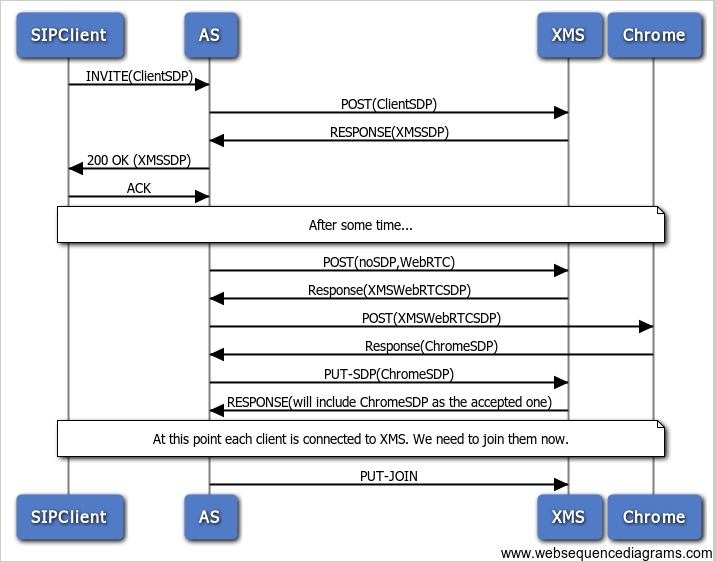
\includegraphics[width=0.95\textwidth,natwidth=610,natheight=642]{figs/sip2xms.png}
  	\caption{Single Call from SIP Client to Browser Client}
  	\label{fig:sip2xms}
\end{figure}

\par The rest of the interfaces for XMS media server on application server is similar as \textit{createXMSCall} interface. \textit{joinXMSCall} interface is made for single call resource join with another single call resource, it is used when a \gls{webrtc} call resource join a \gls{sip} call resource in the prototype system. \textit{updateLocalSDP} is made to update the \gls{sdp} of the call resource on the XMS media server, but it does not work well against the current XMS media server when the \gls{webrtc} call resource is made without \gls{sdp} during the test and development. For this reason, the prototype application server can not use the normal process shown in Figure \ref{fig:sip2xms} when application server got a \gls{sip} \textit{INVITE} message. During the test, after all the process for the \gls{sip} \gls{rtp} session initialization , to create the \gls{webrtc} call resource on XMS media server without \gls{sdp}, it fails to connect with browser client in the \gls{rtp} session. To fix that, the application does the same process for the \gls{webrtc} part as the process shown in Figure \ref{fig:webrtc2xms}. It means that no matter the \gls{webrtc} client is a receiver or a sender of this call request during the establishment, for \gls{webrtc} client itself will treat itself as a sender all the time, then the application server can always get the correct \gls{sdp} from the client to create the \gls{webrtc} call resource on XMS media server. This implementation of fixing solution is based on the WebSocket channels \textit{answer} and \textit{answerInvite} shown at line 61 to line 94 in Code Snippet \ref{code:client_socket} and at line 108 to line 194 in Code Snippet \ref{code:server_socket} with the \textit{self} flag value to see if the client is sender or receiver of the \textit{INVITE} message. This issue is reported to Dialogic team, hope it will be resolved in the future version of XMS media server.

\par \textit{createConference} and \textit{joinConference} are the corresponding interfaces against \textit{createXMSCall} and \textit{joinXMSCall}, they are made for conference resources usage on XMS media server. \textit{deleteXMSCall} and \textit{deleteXMSConference} is the delete function for call resources and conference resources on XMS media server.

\section{Advanced Communication Function Implementation}

\noindent The most exciting reason for combining \gls{webrtc} technology with \gls{sip} \gls{voip} network is there are more advanced communication function could be implemented under the power of web application. There are two main advanced communication functions implemented in prototype system.

\subsection{SMS Messaging}

\par \gls{sms} messaging is required for normal telephone usage. In the prototype system, it is necessary to have \gls{sms} messaging function during the conference if one of the participant is on his mobile phone. The working prototype is shown in Figure \ref{fig:webgui_send_sms}. The implementation is based on \gls{msg} provided by Gintel AS. It is a message service gateway for \gls{sip} clients to send \gls{sms} to other \gls{sip} clients or physical mobile phone. The implementation is shown in Code Snippet \ref{code:msg}. It uses the same \gls{http} Node.js module to implement the \gls{http} request communication with \gls{msg} server.

\par There are two steps to send \gls{sms} message. The first one is to get correct \gls{msg} user credential by providing the correct \textit{loginDto} object. \textit{loginDto} is a \gls{json} object generate with the user name and password from the user. From line 3 to line 44 in Code Snippet \ref{code:msg} is the implementation of this process. At line 28 in Code Snippet \ref{code:msg}, it is shown that if the credential sent to \gls{msg} server is correct, it will return a validate cookie in response data. This cookie will be used for second setup to send \gls{sms} message. From line 46 to line 94 is the implementation of second step, the login credential and cookie need to set in the header fields \textit{login} and \textit{Cookie}(shown at line 59 and 60). Moreover the message string is set in the \gls{http} request body then the \textit{Content-Type} and \textit{Content-Length} in the headers should be set as "application/json" and the length of message string content(it shows at line 57 and line 61).

\subsection{Files Sharing}

\par Because the \gls{rtp} media channel is connected with XMS media server for media  stream exchange, \gls{webrtc} \textit{RTCDataChannel} can not be used in this case. However, consider the prototype system is a real-time communication platform for collaboration working scenario, it is necessary for end point to have some collaboration tool such as files sharing. The screen shoot of file sharing in prototype application is shown in Figure \ref{fig:webgui_file_share_sender} and Figure \ref{fig:webgui_file_share_receiver}.

\begin{figure}
	\centering
    	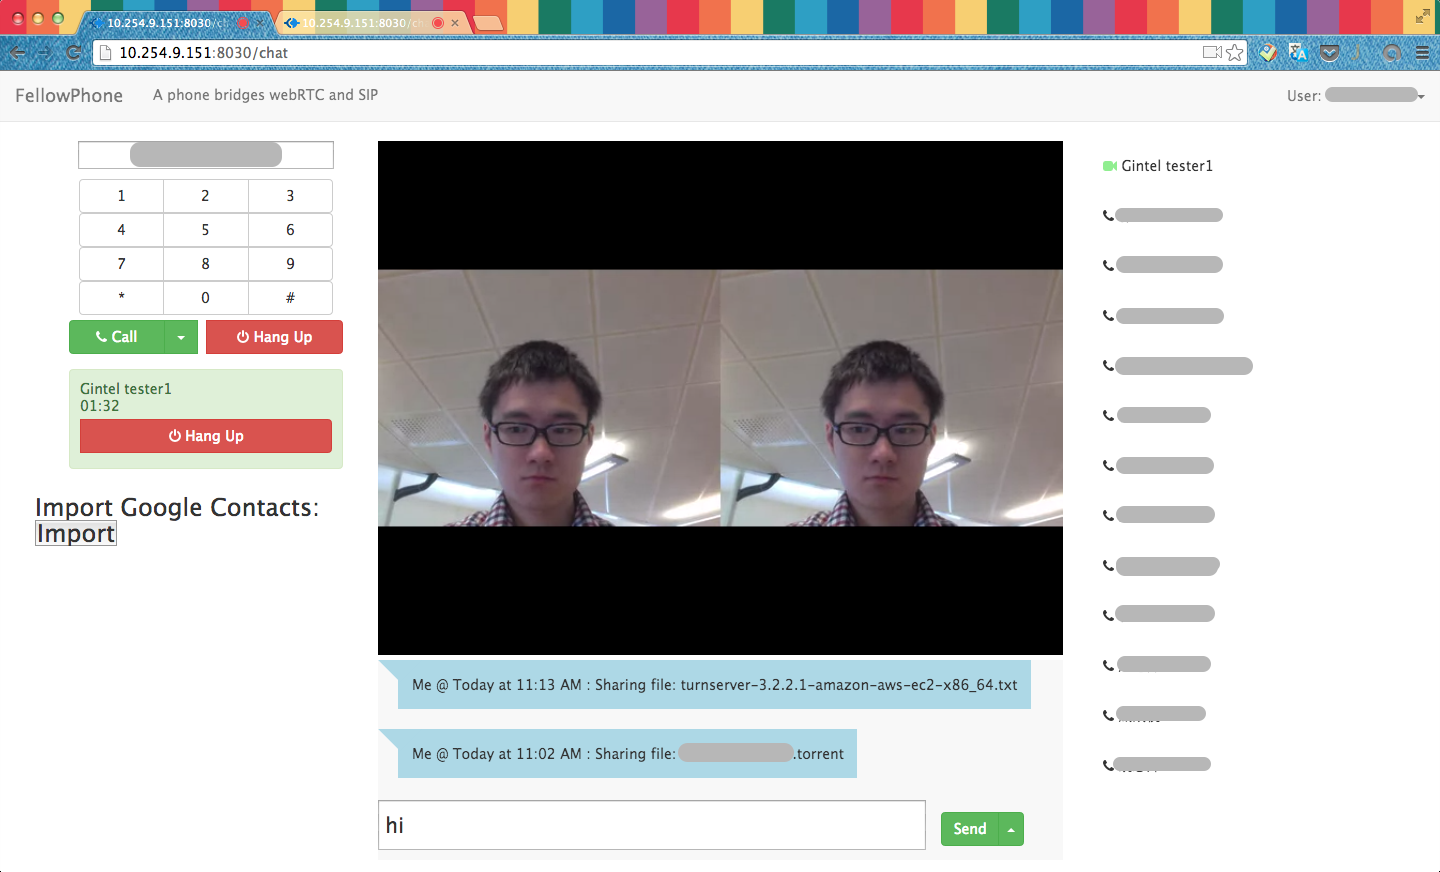
\includegraphics[width=0.85\textwidth,natwidth=610,natheight=642]{figs/webgui_file_share_sender.png}
  	\caption{File Sharing Sender Client}
  	\label{fig:webgui_file_share_sender}
  	    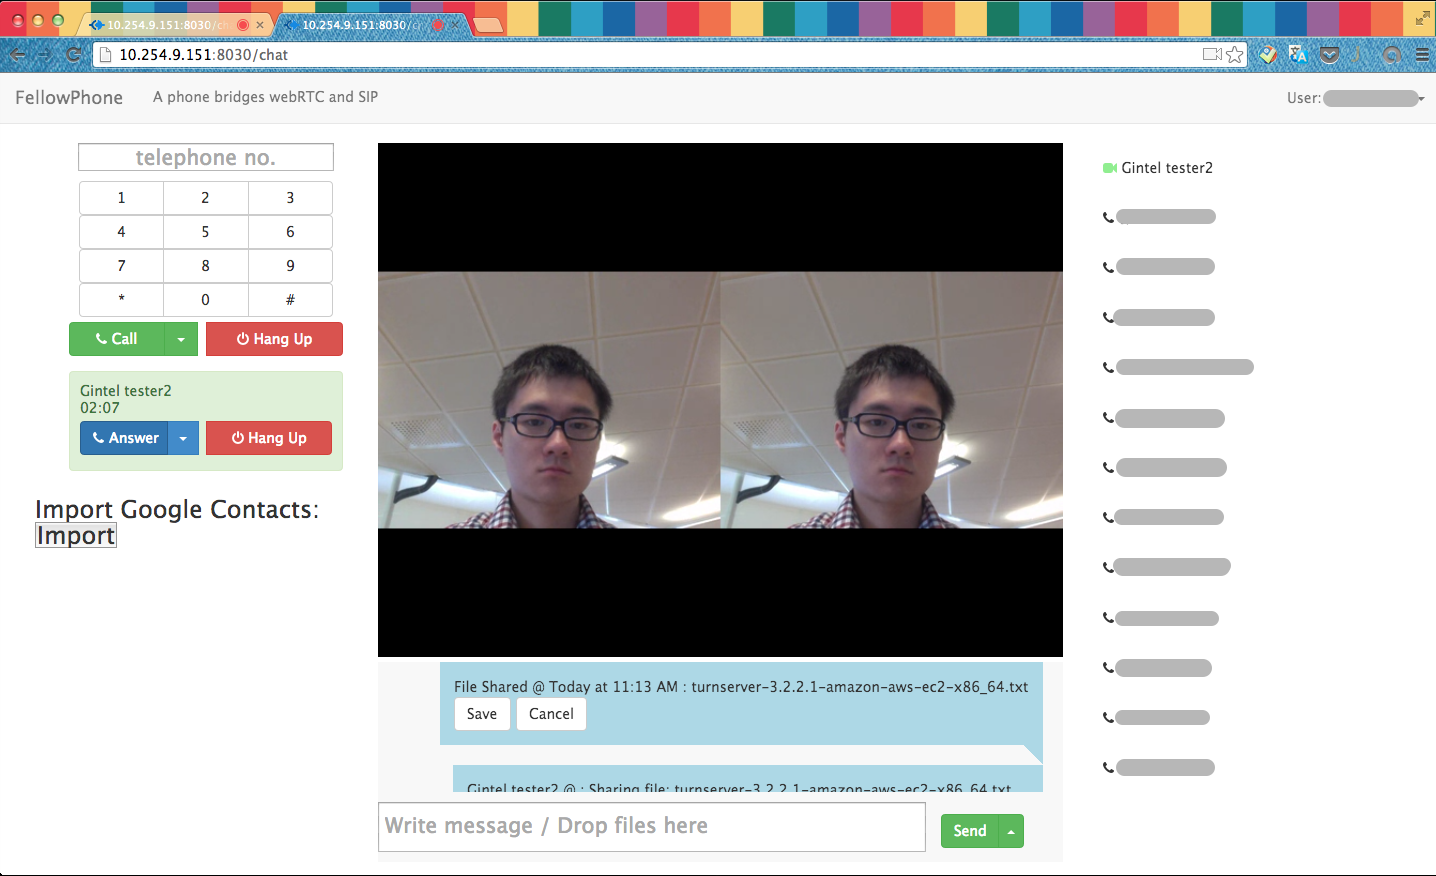
\includegraphics[width=0.85\textwidth,natwidth=610,natheight=642]{figs/webgui_file_share_receiver.png}
  	\caption{File Sharing Receiver Client}
  	\label{fig:webgui_file_share_receiver}
\end{figure}

\par As the screen shoot showed when sender client upload files to the application server, application server will directly share the files with the other clients in current conference session. The receiver client can decide whether the file need to be saved or not.

\par Prototype application uses Delivery.js library to do bidirectional File Transfers For Node.js via Socket.IO. Delivery.js uses Node.js and Socket.IO to make it easy to push files to the client, or send them to the server. Files can be pushed to the client as text (utf-8) or base64 (for images and binary files).\cite{github:deliveryjs} Since it is based on Socket.IO, it has the similar client and server implementation mechanism as Socket.IO. While Delivery.js is more of an experiment, there could be some advantages to using Web Sockets to transfer files. Once a Web Socket connection is established messages (frames) sent between the client and server contain only 2 additional bytes of overhead. In contrast, a traditional \textit{POST} request, and response, may have headers totaling 871 bytes. This could be a significant addition if many files are being sent, and would be even more significant if files are being divided into batches before being sent to the server. When pushing files to the client, the overhead of traditional polling methods provides an even starker contrast to Web Sockets.

\par At line 16 in Code Snippet \ref{code:server_socket}, it declare the \textit{delivery} object using Delivery.js \gls{api} \textit{dl.listen()} with the Socket.IO \textit{socket} object as the argument. From line 643 to line 676 in Code Snippet \ref{code:server_socket} is the server side Delivery.js implementation code. It listens on the 'receive.success' WebSocket channel, when the upload files from client are received successfully the application server will make temporary files for the upload files and push these files to every connected clients in sender's current conference session. For security reasons, the temporary files will be removed from the server when all the pushing process finished.

\par After the files pushed to the client, at line 88 to line 102 in Code Snippet \ref{code:chatboard_ctrl}, the client side implementation will listen the same WebSocket channel 'receive.success'. When there is file message from the application server to the client, the client listener will saved the files in the runtime memory (it is not best solution for files sharing case, the improvement will be discussed in Chapter \ref{chp:future_work}), then let the user decide if these files need to be downloaded or removed.

\par Because Delivery.js sends files in base64\footnote{Base64 is a group of similar binary-to-text encoding schemes that represent binary data in an ASCII string format by translating it into a radix-64 representation. The term Base64 originates from a specific MIME content transfer encoding.\cite{wiki:base64}} encoding format, on the client application, it is necessary to convert base64 encoding string to Web Blob\footnote{A Blob object represents a file-like object of immutable, raw data. Blobs represent data that isn't necessarily in a JavaScript-native format. The File interface is based on Blob, inheriting blob functionality and expanding it to support files on the user's system.\cite{mdn:blob}} data for using the \gls{html5} \gls{w3c} \textit{saveAs()} function. The converting function is implemented at line 22 to line 44 as \textit{b64toBlob()} function, it takes base64 string, content type of the file and slice size (in the prototype case it uses default 512 bit) to convert base64 string data to Web Blob data.

